\section{Proofs and Detailed Derivations}
\label{sec:theory-proofs}

\subsection{Proof of Lemma~\ref{lem:cfg-modes}}
For well-separated modes, $p(\mathbf{x}\mid c)^{1+\lambda} \approx \sum_k \pi_{c,k}^{1+\lambda}\,\mathcal{N}(\mathbf{x};\boldsymbol{\mu}_{c,k},\boldsymbol{\Sigma}_{c,k})^{1+\lambda}$ in each mode's support. Since $\mathcal{N}(\mathbf{x};\boldsymbol{\mu},\boldsymbol{\Sigma})^{1+\lambda} \propto \mathcal{N}(\mathbf{x};\boldsymbol{\mu},\boldsymbol{\Sigma}/(1+\lambda))$ (a Gaussian raised to a power remains Gaussian with rescaled covariance), the result follows. The $p(\mathbf{x})^{-\lambda}$ term contributes a slowly-varying factor that we absorb into the normalization; this is exact when $p(\mathbf{x})$ is uniform and approximate otherwise.

\subsection{Proof of Proposition~\ref{prop:div-cost}}
Substituting $\tilde{\pi}_k = \pi_k^{1+\lambda}/Z$ into the KL divergence yields $D_c(\lambda) = \sum_k \pi_k \log\pi_k - \sum_k \pi_k[(1{+}\lambda)\log\pi_k - \log Z] = \lambda H_c + \log Z$. For (a), $Z(0) = 1$ and $Z'(0) = \sum_k \pi_k \log\pi_k = -H_c$, so $D_c'(0) = H_c + Z'(0)/Z(0) = 0$. For (b), $Z''(0) = \sum_k \pi_k(\log\pi_k)^2$, giving $D_c''(0) = Z''(0) - Z'(0)^2 = \sum_k \pi_k(\log\pi_k)^2 - H_c^2 = \mathrm{Var}_{\boldsymbol{\pi}_c}[\log\pi_k]$. For (c), $\mathrm{Var}[\log\pi_k] = \mathbb{E}[(\log\pi_k)^2] - (\mathbb{E}[\log\pi_k])^2 = \mathbb{E}[(\log\pi_k)^2] - H_c^2$. Since $\log$ is concave, $\mathbb{E}[(\log\pi_k)^2]$ is Schur-convex and $H_c$ is Schur-concave; as the distribution becomes more balanced ($H_c$ increases), both terms converge, driving the variance to zero at maximum entropy (all $\pi_k = 1/K_c$).

\subsection{Proof of Proposition~\ref{prop:opt-lambda}}
By Proposition~\ref{prop:div-cost}, $D_c(\lambda) \approx \frac{1}{2}\sigma_c^2\,\lambda^2$ for small $\lambda$ (using $D_c(0) = D_c'(0) = 0$ and $D_c''(0) = \sigma_c^2$). Substituting into the utility: $U_c(\lambda) \approx v_c + v_c\lambda - \frac{\beta}{2}\sigma_c^2\,\lambda^2$. Setting $U_c'(\lambda) = v_c - \beta\,\sigma_c^2\,\lambda = 0$ yields $\lambda_c^* = v_c / (\beta\,\sigma_c^2)$. The monotonicity claims follow: $\partial\lambda_c^*/\partial v_c = 1/(\beta\,\sigma_c^2) > 0$, and $\partial\lambda_c^*/\partial H_c = -v_c/(\beta\,\sigma_c^4)\cdot\partial\sigma_c^2/\partial H_c > 0$ since $\partial\sigma_c^2/\partial H_c < 0$ by Proposition~\ref{prop:div-cost}(c).

\subsection{Proof of Theorem~\ref{thm:adaptivity-gap}}
Since $U_c(\lambda)$ is a concave quadratic in $\lambda$ (to second order), $U_c(\lambda) = U_c(\lambda_c^*) - \frac{\beta\sigma_c^2}{2}(\lambda - \lambda_c^*)^2$. Averaging over classes and noting $U_c(\lambda_c^*) - U_c(\bar\lambda) = \frac{\beta\sigma_c^2}{2}(\bar\lambda - \lambda_c^*)^2$ yields the adaptivity gap. Non-negativity follows from the squared term; equality holds iff $\lambda_c^* = \bar\lambda$ for all $c$.

\subsection{Proof of Lemma~\ref{lem:sep-invariance}}
By Lemma~\ref{lem:cfg-modes}, the effective mode weights $\tilde{\pi}_{c,k}(\lambda) = \pi_{c,k}^{1+\lambda}/\sum_j \pi_{c,j}^{1+\lambda}$ depend solely on the intra-class mode proportions $\boldsymbol{\pi}_c$. The diversity cost $D_c(\lambda)$ (Proposition~\ref{prop:div-cost}) is therefore a function of $\boldsymbol{\pi}_c$ alone. Since $\lambda_c^* \approx v_c / (\beta\,\sigma_c^2)$ (Proposition~\ref{prop:opt-lambda}) involves only $v_c$ (intra-class variance) and $\sigma_c^2$ (a function of $\boldsymbol{\pi}_c$), inter-class separability does not enter. The $p(\mathbf{x})^{-\lambda}$ term in CFG involves the marginal $p(\mathbf{x}) = \sum_{c'} p(c')\,p(\mathbf{x}|c')$, which depends on all classes; however, for well-separated classes, this term contributes a class-dependent constant that is absorbed into the normalization (Lemma~\ref{lem:cfg-modes}), leaving the mode structure---and hence the optimal $\lambda_c^*$---unaffected by inter-class geometry.

\subsection{Remark on Assumptions}
The well-separated modes assumption (Lemma~\ref{lem:cfg-modes}) is an idealization; in practice, modes may overlap and the $p(\mathbf{x})^{-\lambda}$ term introduces inter-class effects. However, the qualitative predictions---that optimal $\lambda$ increases with $v_c$ and $H_c$, that separability is irrelevant, and that the adaptivity gap grows with class heterogeneity---are robust to relaxation of this assumption, as confirmed by experiments across datasets, architectures, and scales (Sections~\ref{sec:experiments}--\ref{sec:dd-baselines}).

\subsection{From Theory to Implementation}
\label{sec:theory-impl}
Proposition~\ref{prop:opt-lambda} predicts $\lambda_c^* \propto v_c / \sigma_c^2$, which is linear in $v_c$ and entropy-dependent through $\sigma_c^2$. The implementation uses a sigmoid mapping $\rho_c = \sigma(s \cdot (0.5\hat{H}_c + 0.5\hat{v}_c) - c_0)$ followed by $\lambda_c = 0.06\,\rho_c$, which is not a direct instantiation of the linear formula. The sigmoid serves two practical purposes: it bounds $\lambda_c \in [0, 0.06]$ to prevent over-guidance (addressing the small-$\lambda$ regime where the theory is valid), and it provides a smooth, monotonic mapping from the complexity score to the guidance scale that is robust to normalization choices. The key theoretical predictions---that $\lambda_c$ should be increasing in both $H_c$ and $v_c$, and independent of separability---are preserved by the sigmoid mapping since it is monotonic in its argument. The linear prediction from the theory provides the \emph{qualitative} design rationale (which factors to include, which to exclude), while the sigmoid provides the \emph{quantitative} robustness needed for practical deployment.

\subsection{Quantitative Validation of Theorem~\ref{thm:adaptivity-gap}}
We empirically validate the adaptivity gap prediction by measuring mode structure heterogeneity across datasets of varying class count (\Cref{fig:theorem1-fit}). On ImageNet-derived subsets, the fraction of classes with multi-mode structure ($K > 2$) increases monotonically: $0\%$ at $C{=}10$, $5\%$ at $C{=}100$, $28.5\%$ at $C{=}200$, and $60\%$ at $C{=}1000$, tracking the increasing diversity of mode structures. The actual CAGS gain increases in parallel: $0\%$ at $C{=}10$, $+2.65\%$ at $C{=}100$, $+3.30\%$ at $C{=}200$, $+3.58\%$ at $C{=}1000$. Notably, the 10-class datasets ImageNette ($+5.28\%$) and ImageWoof ($+1.12\%$) show varying gains despite having $K{=}2$ for all classes, indicating that intra-class variance heterogeneity alone can drive the adaptivity gap.

\begin{figure}[ht]
\centering
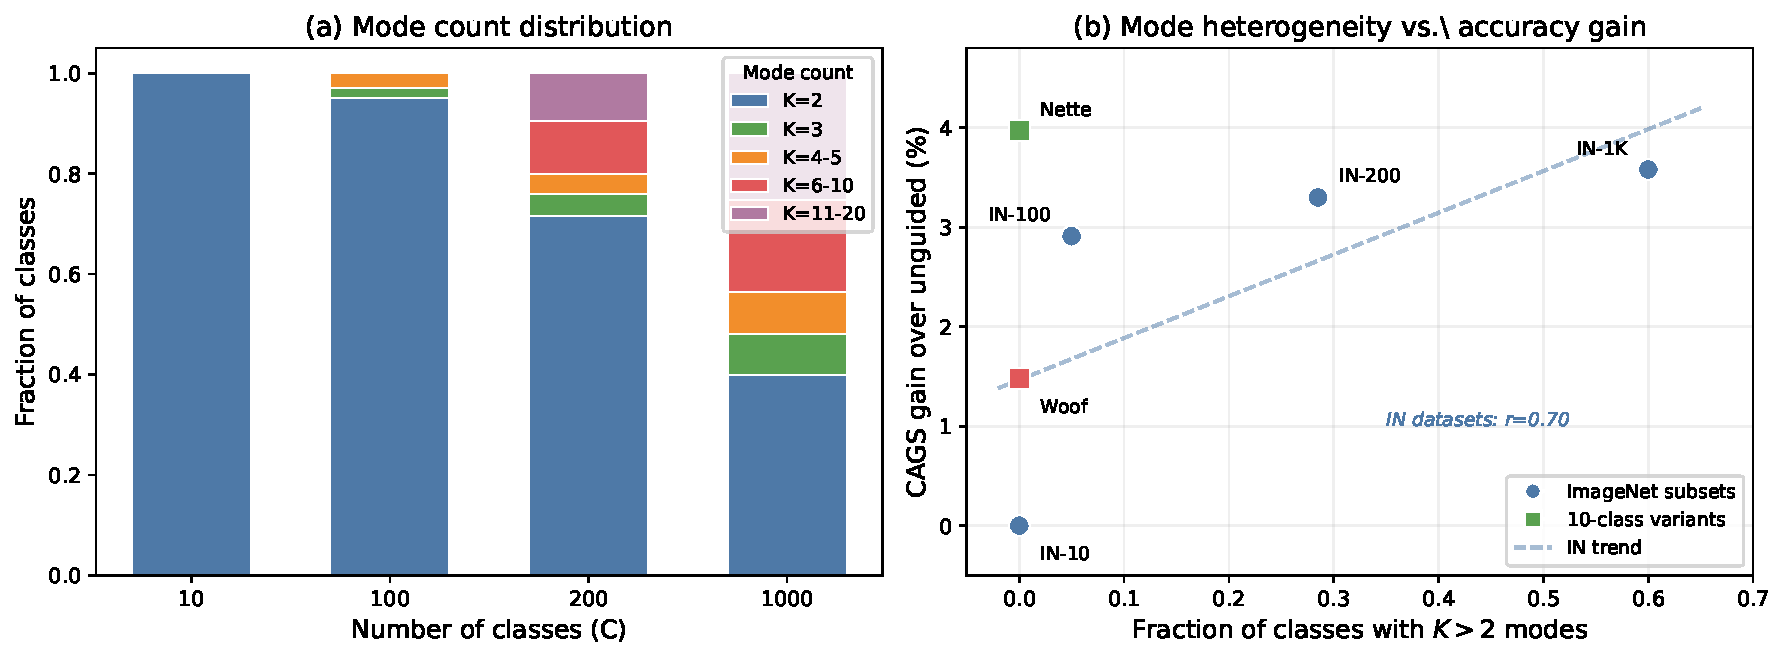
\includegraphics[width=\columnwidth]{figures/theorem1_fit.pdf}
\caption{Quantitative validation of Theorem~\ref{thm:adaptivity-gap}. (a)~Distribution of mode counts ($K$) across ImageNet subsets with increasing class count. (b)~Mode heterogeneity (fraction of classes with $K > 2$) vs.\ actual CAGS accuracy gain.}
\label{fig:theorem1-fit}
\end{figure}

\section{\ags{} Framework and Sampling Algorithm}
\label{sec:algorithm}

\begin{algorithm}[ht]
\caption{\ags{} Sampling (CAGS core)}
\label{alg:ags}
\begin{algorithmic}[1]
\Require Frozen DiT $\epsilon_\theta$, class $c$, complexity cache $\{\rho_{c'}\}_{c'=1}^C$
\Ensure Synthetic image $\mathbf{x}_0$
\State $\lambda_c \gets \lambda_{\min} + (\lambda_{\max} - \lambda_{\min}) \cdot \rho_c$ \Comment{CAGS per-class guidance}
\State $\mathbf{x}_{t_{\text{start}}} \sim \mathcal{N}(\mathbf{0}, \mathbf{I})$
\For{$t = t_{\text{start}}, t_{\text{start}}-1, \ldots, 1$}
    \State \textcolor{gray}{// Optional: $\lambda_t \gets \textsc{TAGS}(\lambda_c, t)$ \Comment{TAGS (not recommended)}}
    \State $\tilde{\epsilon} \gets (1 + \lambda_c)\,\epsilon_\theta(\mathbf{x}_t, t, c) - \lambda_c\,\epsilon_\theta(\mathbf{x}_t, t, \varnothing)$
    \State $\mathbf{x}_{t-1} \gets \text{DenoiseStep}(\mathbf{x}_t, \tilde{\epsilon}, t)$
\EndFor
\State \Return $\mathbf{x}_0$
\end{algorithmic}
\end{algorithm}
